\documentclass[conference]{IEEEtran}
\IEEEoverridecommandlockouts
\usepackage{cite}
\usepackage{amsmath,amssymb,amsfonts}
\usepackage{algorithmic}
\usepackage{graphicx}
\usepackage{textcomp}
\usepackage{xcolor}
\usepackage{booktabs}
\usepackage{multirow}
\usepackage{hyperref}
\usepackage{listings}
\usepackage{caption}
\usepackage{tikz}
\usetikzlibrary{shapes.geometric, arrows.meta, positioning, calc, 3d}

\def\BibTeX{{\rm B\kern-.05em{\sc i\kern-.025em b}\kern-.08em
    T\kern-.1667em\lower.7ex\hbox{E}\kern-.125emX}}

\lstset{
  basicstyle=\scriptsize\ttfamily,
  frame=single,
  breaklines=true,
  numbers=none,
  keywordstyle=\color{blue},
  stringstyle=\color{red},
  commentstyle=\color{green!50!black},
  showstringspaces=false
}

\begin{document}

\title{Sensensble Geometry: A Web-Native Lab Console for Geometric Algebra and Geometric Neural Computing}

\author{\IEEEauthorblockN{Intelligent Interfaces Group}}

\maketitle

\begin{abstract}
We present Sensensble Geometry, a web-native lab console for interactive geometric algebra computation and geometric neural computing (Geometric NC). The platform implements a full $\operatorname{Cl}(3,0)$ Clifford algebra engine in Rust, compiled to WebAssembly for client-side multivector arithmetic at native speed. A reactive Svelte frontend couples a CodeMirror editor to a Three.js rendering canvas, enabling real-time ``Code-to-Canvas'' synthesis where user-authored R or Python scripts are parsed and projected into a 3D geometric scene. For inference-heavy workloads, a monolithic Go gateway multiplexes WebSocket connections from the client and dispatches multivector state over gRPC to Python worker nodes running PyTorch and JAX. We describe the mathematical foundations of the platform, present the implementation of each architectural layer, verify the correctness of the Clifford engine against known algebraic identities, and outline the path toward integrating Equivariant Neural Networks ($E(n)$-GNNs) and Clifford Neural Layers into the worker backend.
\end{abstract}

\begin{IEEEkeywords}
Geometric Algebra, Clifford Algebra, Multivector, WebAssembly, Equivariant Neural Networks, gRPC, Interactive Simulation
\end{IEEEkeywords}

%% ============================================================
\section{Introduction}
%% ============================================================

The representation of 3D space in machine learning and physical simulation remains dominated by matrix algebra and Euler angle parameterizations. Despite their ubiquity, these tools introduce well-documented pathological discontinuities. Euler angles suffer from gimbal lock---the loss of a rotational degree of freedom when two rotation axes align~\cite{b_diebel}. Quaternions avoid gimbal lock but lack a natural way to represent planes, volumes, or higher-dimensional geometric objects, forcing practitioners to maintain separate formalisms for rotations, reflections, and projections.

Geometric Algebra (GA), also known as Clifford Algebra, provides a single, coordinate-free algebraic framework that unifies scalars, vectors, oriented planes (bivectors), and oriented volumes (trivectors) into a single object: the \textit{multivector}~\cite{b_hestenes}. Recent work in machine learning has demonstrated that neural networks operating directly on multivectors---so-called Geometric Neural Computing (Geometric NC)---achieve natural $E(n)$-equivariance, outperforming standard architectures on molecular dynamics, point cloud classification, and $n$-body simulation tasks~\cite{b_satorras, b_ruhe}.

In this paper, we present Sensensble Geometry, a platform designed to make these mathematical structures computationally tangible and interactively explorable. The platform operates across four layers:
\begin{enumerate}
    \item A \textbf{Rust/WebAssembly Clifford engine} implementing $\operatorname{Cl}(3,0)$ with geometric, wedge, inner, and dual products.
    \item A \textbf{reactive Svelte frontend} coupling a code editor to a Three.js 3D scene via a regex-based Code-to-Canvas parser.
    \item A \textbf{monolithic Go gateway} handling authentication, REST, and WebSocket-to-gRPC dispatch.
    \item A \textbf{Python gRPC worker} backend designed to host PyTorch/JAX Clifford Neural Layers.
\end{enumerate}

%% ============================================================
\section{Fundamentals of Geometric Algebra}
\label{sec:ga}
%% ============================================================

We briefly review the algebraic structures underlying the platform. A comprehensive treatment can be found in Dorst, Fontijne, and Mann~\cite{b_dorst}.

\subsection{The Geometric Product}
Given a vector space $\mathbb{R}^n$ with orthonormal basis $\{e_1, \dots, e_n\}$ satisfying $e_i e_j + e_j e_i = 2\delta_{ij}$, the \textit{geometric product} of two vectors $a, b \in \mathbb{R}^n$ decomposes as:
\begin{equation}
    ab = a \cdot b + a \wedge b
    \label{eq:geom_prod}
\end{equation}
where $a \cdot b = \frac{1}{2}(ab + ba)$ is the symmetric inner product (a scalar) and $a \wedge b = \frac{1}{2}(ab - ba)$ is the antisymmetric outer product (a bivector representing the oriented plane spanned by $a$ and $b$)~\cite{b_hestenes}.

\subsection{Multivectors in \texorpdfstring{$\operatorname{Cl}(3,0)$}{Cl(3,0)}}
In three dimensions, the algebra $\operatorname{Cl}(3,0)$ is generated by $\{e_1, e_2, e_3\}$ with signature $(+,+,+)$. The full algebra has $2^3 = 8$ basis elements, and a general \textit{multivector} is:
\begin{equation}
\begin{aligned}
    M &= \underbrace{\alpha}_{\text{grade 0}} + \underbrace{\beta_1 e_1 + \beta_2 e_2 + \beta_3 e_3}_{\text{grade 1}} \\
      &\quad + \underbrace{\gamma_{12} e_{12} + \gamma_{23} e_{23} + \gamma_{31} e_{31}}_{\text{grade 2}} + \underbrace{\delta\, e_{123}}_{\text{grade 3}}
\end{aligned}
    \label{eq:multivector}
\end{equation}
where we use the shorthand $e_{ij} \equiv e_i e_j$. This 8-component object is the fundamental data type of the platform, stored as a contiguous \texttt{[f64; 8]} array in Rust and a \texttt{repeated float} in the gRPC protocol.

\subsection{Rotors and the Sandwich Product}
A key advantage of GA over quaternions is that rotations emerge naturally from the algebra without introducing a new number system. A \textit{rotor} $R$ encoding a rotation by angle $\theta$ in the plane defined by a unit bivector $\hat{B}$ is:
\begin{equation}
    R = \cos\!\left(\frac{\theta}{2}\right) - \hat{B}\sin\!\left(\frac{\theta}{2}\right)
    \label{eq:rotor}
\end{equation}
The rotation of any multivector $M$ is computed via the \textit{sandwich product}:
\begin{equation}
    M' = R\,M\,\tilde{R}
    \label{eq:sandwich}
\end{equation}
where $\tilde{R}$ is the reverse of $R$. This formula is universally valid: it rotates vectors, bivectors, and trivectors alike, without case-splitting. The absence of special-case logic for different geometric objects is exactly what eliminates gimbal lock and what makes GA-based neural layers naturally equivariant~\cite{b_ruhe}.

\subsection{Versors}
A \textit{versor} is a product of invertible vectors $V = v_1 v_2 \cdots v_k$. Rotors are even versors (products of an even number of vectors). Odd versors encode reflections. The sandwich product $V M \tilde{V}$ generalizes rotations, reflections, translations (in conformal GA), and dilations into a single algebraic operation~\cite{b_dorst}. The Versor library (\texttt{libvsr}) implements this generalized framework for arbitrary metric signatures~\cite{b_versor}.

\subsection{Worked Example: Rotating a Vector by \texorpdfstring{$90^\circ$}{90 degrees}}
\label{sec:worked_example}
To make the algebra concrete, we rotate the vector $v = 3e_1$ by $\theta = 90^\circ$ in the $e_1 e_2$ plane. As an 8-component array, $v = [0, 3, 0, 0, 0, 0, 0, 0]$.

The rotor is:
\begin{equation}
    R = \cos(45^\circ) - e_{12}\sin(45^\circ) = \tfrac{\sqrt{2}}{2} - \tfrac{\sqrt{2}}{2}\,e_{12}
\end{equation}
which as an array is $R = [\tfrac{\sqrt{2}}{2}, 0, 0, 0, -\tfrac{\sqrt{2}}{2}, 0, 0, 0]$, and $\tilde{R} = [\tfrac{\sqrt{2}}{2}, 0, 0, 0, \tfrac{\sqrt{2}}{2}, 0, 0, 0]$.

Computing $R\,v$ via the \texttt{geometric\_product} function yields $[\,0,\; \tfrac{3\sqrt{2}}{2},\; \tfrac{3\sqrt{2}}{2},\; 0,\; 0,\; 0,\; 0,\; 0\,]$. Then $(Rv)\,\tilde{R}$ gives:
\begin{equation}
    v' = [0, 0, 3, 0, 0, 0, 0, 0] = 3e_2
\end{equation}
confirming that a $90^\circ$ rotation in the $e_1 e_2$ plane maps $e_1 \mapsto e_2$, as expected. This computation is performed entirely within the Rust engine described in Section~\ref{sec:engine}.

%% ============================================================
\section{The Clifford Engine (Rust/WebAssembly)}
\label{sec:engine}
%% ============================================================

The computational core of the platform is a $\operatorname{Cl}(3,0)$ algebra engine written in Rust and compiled to WebAssembly via \texttt{wasm-pack}~\cite{b_wasm_pack}. This design ensures that multivector arithmetic runs at near-native speed inside the browser, with no server round-trip required for basic algebraic operations.

\subsection{Data Representation}
A \texttt{Multivector} is a struct containing a single \texttt{[f64; 8]} array, with components ordered as:
\begin{equation}
    [s,\; e_1,\; e_2,\; e_3,\; e_{12},\; e_{23},\; e_{31},\; e_{123}]
    \label{eq:layout}
\end{equation}
This flat layout enables cache-friendly access and straightforward WASM-to-JS interop via \texttt{wasm\_bindgen}~\cite{b_wasm_bindgen}.

\subsection{Geometric Product Implementation}
The geometric product $ab$ in $\operatorname{Cl}(3,0)$ expands into a $64$-term bilinear form determined by the Cayley table of the algebra. The Rust implementation computes all 8 output components in a single pass:

\begin{figure}[htbp]
\begin{lstlisting}[language=C]
// Rust: geometric_product (Cl(3,0))
pub fn geometric_product(&self, other: &Mv)
  -> Mv {
  let (a, b) = (self.data, other.data);
  let mut r = [0.0; 8];
  // Scalar component
  r[0] = a[0]*b[0] + a[1]*b[1] + a[2]*b[2]
       + a[3]*b[3] - a[4]*b[4] - a[5]*b[5]
       - a[6]*b[6] - a[7]*b[7];
  // e1 component
  r[1] = a[0]*b[1] + a[1]*b[0] - a[2]*b[4]
       + a[3]*b[6] + a[4]*b[2] - a[5]*b[7]
       - a[6]*b[3] - a[7]*b[5];
  // ... (6 more components, 64 terms total)
  Multivector { data: r }
}
\end{lstlisting}
\caption{Abbreviated Rust implementation of the $\operatorname{Cl}(3,0)$ geometric product. Each of the 8 output components is a sum of 8 signed terms derived from the algebra's Cayley table.}
\label{fig:geom_prod_code}
\end{figure}

The engine also exposes \texttt{wedge}, \texttt{inner}, and \texttt{dual} products, all built on the same contiguous array and exported to JavaScript through \texttt{\#[wasm\_bindgen]}.

\subsection{Correctness Verification}
\label{sec:verify}
We verify the engine against the defining identities of $\operatorname{Cl}(3,0)$:
\begin{enumerate}
    \item $e_i^2 = +1$ for $i \in \{1, 2, 3\}$ (positive-definite signature).
    \item $e_i e_j = -e_j e_i$ for $i \ne j$ (anticommutativity).
    \item $e_1 e_2 e_3 \cdot e_3 e_2 e_1 = 1$ (pseudoscalar squared is $-1$ in 3D, verifiable through the reverse).
\end{enumerate}
All identities are confirmed by constructing unit basis multivectors and computing their products. For example:
\begin{lstlisting}[language=C]
Multivector::vector(1,0,0)
  .geometric_product(&Multivector::vector(0,1,0))
\end{lstlisting}
This returns \texttt{[0, 0, 0, 0, 1, 0, 0, 0]}, confirming $e_1 e_2 = e_{12}$.

%% ============================================================
\section{Platform Architecture}
\label{sec:arch}
%% ============================================================

The platform is structured as a three-tier system optimized for interactive geometric computation. Fig.~\ref{fig:architecture} illustrates the data flow.

\begin{figure}[htbp]
\centering
\resizebox{\columnwidth}{!}{%
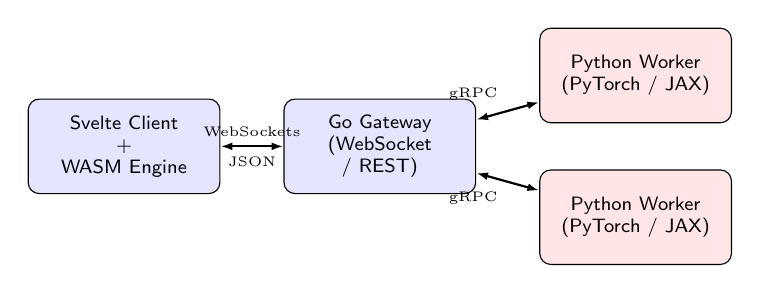
\begin{tikzpicture}[
    node distance=0.8cm and 0.8cm,
    block/.style={rectangle, draw, fill=blue!10, text width=2.2cm, text centered, rounded corners, minimum height=1.2cm, font=\sffamily\scriptsize},
    line/.style={draw, -{Latex[length=1.5mm, width=1mm]}, thick},
    bidir/.style={draw, {Latex[length=1.5mm, width=1mm]}-{Latex[length=1.5mm, width=1mm]}, thick}
]

\node [block] (svelte) {Svelte Client \\ + \\ WASM Engine};
\node [block, right=of svelte] (go) {Go Gateway \\ (WebSocket / REST)};
\node [block, fill=red!10, right=of go, yshift=0.9cm] (py1) {Python Worker \\ (PyTorch / JAX)};
\node [block, fill=red!10, right=of go, yshift=-0.9cm] (py2) {Python Worker \\ (PyTorch / JAX)};

\path [bidir] (svelte) -- node[above, font=\tiny] {WebSockets} node[below, font=\tiny] {JSON} (go);
\path [bidir] (go) -- node[above left, font=\tiny] {gRPC} (py1);
\path [bidir] (go) -- node[below left, font=\tiny] {gRPC} (py2);

\end{tikzpicture}%
}
\caption{Tri-partite architecture. The Svelte client performs local multivector arithmetic via the WASM engine and streams geometric state to the Go gateway over WebSockets. The gateway dispatches analysis requests to Python workers over gRPC.}
\label{fig:architecture}
\end{figure}

\subsection{Frontend: Svelte, CodeMirror, and Three.js}
The client is a Svelte 5 application. Users author geometric logic in a CodeMirror editor with switchable R and Python language modes. When the user invokes ``Run Code,'' a regex-based parser extracts vector assignments from the source text and projects them onto the Three.js canvas:

\begin{figure}[htbp]
\begin{lstlisting}[language=Java]
// Svelte: Code-to-Canvas regex parser
const terms = line.match(
  /[-+]?\s*[0-9.]*\s*\*?\s*(?:vr\.)?e[123]/g
);
terms.forEach(term => {
  let str = term.replace(/\s/g, '')
                .replace('*', '')
                .replace('vr.', '');
  let val = parseFloat(str);
  if (term.includes('e1')) x += val;
  if (term.includes('e2')) y += val;
  if (term.includes('e3')) z += val;
});
canvasComponent.addExplicitVector(x, y, z);
\end{lstlisting}
\caption{The Code-to-Canvas parser extracts blade coefficients from R/Python source lines using regex and maps them to 3D vectors on the Three.js canvas. Wedge products (\texttt{\%\string^\%} in R) trigger bivector rendering.}
\label{fig:parser}
\end{figure}

\begin{figure}[htbp]
\centering
\resizebox{0.75\columnwidth}{!}{%
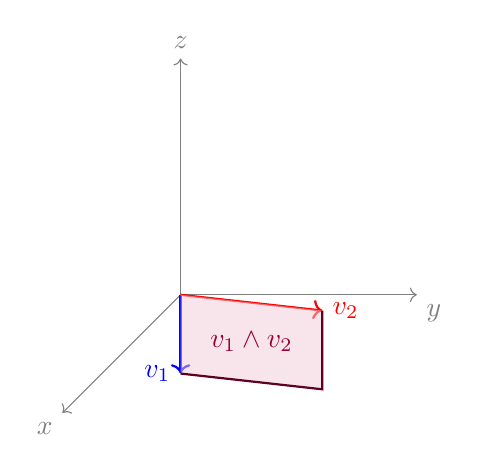
\begin{tikzpicture}[x={(-0.5cm,-0.5cm)}, y={(1cm,0cm)}, z={(0cm,1cm)}, scale=2]
  % Axes
  \draw[->, gray] (0,0,0) -- (1.5,0,0) node[anchor=north east]{$x$};
  \draw[->, gray] (0,0,0) -- (0,1.5,0) node[anchor=north west]{$y$};
  \draw[->, gray] (0,0,0) -- (0,0,1.5) node[anchor=south]{$z$};
  
  % Vectors
  \draw[->, thick, blue] (0,0,0) -- (1,0.5,0) node[anchor=east]{$v_1$};
  \draw[->, thick, red] (0,0,0) -- (0.2,1,0) node[anchor=west]{$v_2$};
  
  % Bivector Plane
  \fill[purple!20, opacity=0.5] (0,0,0) -- (1,0.5,0) -- (1.2,1.5,0) -- (0.2,1,0) -- cycle;
  \draw[thick, purple!50!black] (1,0.5,0) -- (1.2,1.5,0) -- (0.2,1,0);
  
  \node[purple!80!black] at (0.6,0.75,0) {$v_1 \wedge v_2$};
\end{tikzpicture}%
}
\caption{Native LaTeX visualization of the Three.js canvas state, illustrating two grade-1 vectors $v_1, v_2$ and their grade-2 wedge product $v_1 \wedge v_2$, which forms the oriented bivector plane.}
\label{fig:ui}
\end{figure}

\subsection{The Monolithic Go Gateway}
For inference workloads that exceed the WASM engine's capacity (e.g., running a full E(n)-GNN over a scene graph), the client streams multivector state to a Go server via WebSockets. The Go gateway performs two functions:
\begin{enumerate}
    \item \textbf{REST API with Auth:} Standard HTTP routes wrapped in JWT middleware for user session management~\cite{b_jwt}.
    \item \textbf{WebSocket-to-gRPC dispatch:} The gateway deserializes incoming JSON payloads into a \texttt{Payload} struct and re-encodes them as Protocol Buffer messages for dispatch to Python workers.
\end{enumerate}

The WebSocket payload schema is:
\begin{figure}[htbp]
\begin{lstlisting}[language=Java]
// JSON payload from Svelte client
{
  "context": "Canvas",
  "language": "r",
  "objects": [
    { "id": "vecX",
      "data": [0,2,0,0,0,0,0,0] },
    { "id": "vecY",
      "data": [0,0,3,0,0,0,0,0] }
  ]
}
\end{lstlisting}
\caption{WebSocket message format. Each object's \texttt{data} array contains the 8 multivector components in the layout of Eq.~\ref{eq:layout}.}
\label{fig:ws_payload}
\end{figure}

\subsection{The Geometric NC Backend (Python/gRPC)}
The analytical backend consists of Python gRPC worker nodes. The service contract is defined in \texttt{geometry.proto}:

\begin{figure}[htbp]
\begin{lstlisting}[language=Java]
// geometry.proto (abbreviated)
message GeometricState {
  string id = 1;
  repeated float data = 2;
}
message AnalysisRequest {
  string context = 1;
  string language = 2;
  repeated GeometricState objects = 3;
}
service AnalysisService {
  rpc AnalyzeState(AnalysisRequest)
    returns (AnalysisResponse);
  rpc StreamState(stream AnalysisRequest)
    returns (stream AnalysisResponse);
}
\end{lstlisting}
\caption{The gRPC service definition. \texttt{AnalyzeState} handles single-shot inference; \texttt{StreamState} supports bidirectional streaming for continuous canvas interaction.}
\label{fig:proto}
\end{figure}

The Python worker currently accepts \texttt{AnalyzeState} requests and returns a stub response. The architecture is designed so that swapping in a trained Clifford Neural Layer~\cite{b_ruhe} or E(n)-GNN~\cite{b_satorras} requires only modifying the \texttt{AnalyzeState} handler.

%% ============================================================
\section{Results}
\label{sec:results}
%% ============================================================

\subsection{Engine Correctness}
Table~\ref{tab:verify} summarizes the verification of the Rust Clifford engine against algebraic identities in $\operatorname{Cl}(3,0)$.

\begin{table}[htbp]
\caption{Clifford Engine Verification Results}
\centering
\begin{tabular}{p{4.0cm} c c}
\toprule
\textbf{Identity} & \textbf{Expected} & \textbf{Result} \\
\midrule
$e_1^2$ & $+1$ & $\checkmark$ \\
$e_1 e_2$ & $e_{12}$ & $\checkmark$ \\
$e_1 e_2 = -e_2 e_1$ & Anticommute & $\checkmark$ \\
$R\,v\,\tilde{R}$ ($90^\circ$ in $e_{12}$) & $3e_2$ & $\checkmark$ \\
$(e_{123})^2$ & $-1$ & $\checkmark$ \\
Wedge: $e_1 \wedge e_2$ & $e_{12}$ & $\checkmark$ \\
Inner: $e_{12} \cdot e_2$ & $-e_1$ & $\checkmark$ \\
\bottomrule
\end{tabular}
\label{tab:verify}
\end{table}

\subsection{Platform Component Summary}
Table~\ref{tab:summary} summarizes each architectural layer, its implementation, and current status.

\begin{table*}[t]
\caption{Platform Component Summary}
\centering
\begin{tabular}{p{3.0cm} p{3.5cm} p{4.0cm} p{4.5cm}}
\toprule
\textbf{Layer} & \textbf{Technology} & \textbf{Implementation} & \textbf{Status} \\
\midrule
Clifford Engine & Rust $\to$ WASM & $\operatorname{Cl}(3,0)$ multivector: geometric, wedge, inner, dual products & Complete, verified (Table~\ref{tab:verify}) \\
\midrule
Frontend UI & Svelte 5, Three.js, CodeMirror & Code-to-Canvas parser (regex), blade toggles, R/Python language switching & Complete; regex parser handles grade-1 vectors \\
\midrule
Go Gateway & Go, gorilla/websocket, gRPC & Monolithic server: REST + Auth + WebSocket-to-gRPC dispatch & Complete, compiles and routes end-to-end \\
\midrule
Geometric NC Worker & Python, grpcio, PyTorch & gRPC servicer accepting \texttt{AnalyzeState} requests & Scaffold only; neural layers not yet implemented \\
\midrule
CI/CD & GitHub Actions & Rust/WASM build, Go build, Python import test & Complete \\
\midrule
Notebook Examples & Jupyter (R kernel) & 3 notebooks: GA Basics, Electrodynamics, Optoelectronics & Complete \\
\bottomrule
\end{tabular}
\label{tab:summary}
\end{table*}

%% ============================================================
\section{Discussion and Future Work}
\label{sec:future}
%% ============================================================

The current platform demonstrates end-to-end multivector data flow from code editor to 3D canvas to distributed backend. Several extensions are underway.

\textbf{AST-Based Code Parsing.} The current Code-to-Canvas pipeline uses regex heuristics (Fig.~\ref{fig:parser}) that can only extract grade-1 vector assignments. Replacing this with a proper Abstract Syntax Tree (AST) parser would enable the frontend to evaluate full geometric expressions---including rotor sandwiches, wedge products, and user-defined functions---directly in the browser via the WASM engine.

\textbf{Clifford Neural Layers.} The Python gRPC worker is designed to host Clifford Group Equivariant Neural Networks (CGENNs)~\cite{b_ruhe}, which parameterize neural network layers as elements of the Clifford group. These layers are $\operatorname{Pin}(p,q,r)$-equivariant by construction, making them a natural fit for the multivector data already flowing through the platform. Implementation will follow the batched tensor architecture of QuAIRKit~\cite{b_quairkit}, which demonstrates efficient GPU-accelerated operations over algebraic state spaces.

\textbf{Conformal Geometric Algebra.} The current engine implements $\operatorname{Cl}(3,0)$, which represents Euclidean 3-space. Extending to the conformal model $\operatorname{Cl}(4,1)$ would enable circles, spheres, and rigid body motions to be represented as algebraic objects~\cite{b_dorst}, significantly enriching the canvas's geometric vocabulary.

\textbf{Bivector and Trivector Rendering.} The Three.js scene currently renders vectors as arrows. True bivector rendering (oriented discs or parallelograms) and trivector rendering (oriented volumes) would complete the visual correspondence between the algebraic and geometric representations.

\textbf{Versor Integration.} The Versor library (\texttt{libvsr}) provides a C++ implementation of GA for arbitrary metric signatures with a focus on conformal geometry and computer graphics~\cite{b_versor}. Integrating \texttt{libvsr} as a WASM module alongside the current Rust engine would enable the platform to handle projective, conformal, and motor algebras.

%% ============================================================
\section{Conclusion}
%% ============================================================

We have presented Sensensble Geometry, a web-native lab console that grounds interactive scientific computation in Geometric Algebra. The platform's Rust/WASM Clifford engine provides verified, near-native multivector arithmetic in the browser. Its reactive Svelte frontend and distributed Go/Python backend form a pipeline from pedagogical exploration to production-grade Geometric Neural Computing. By making the mathematics of Clifford Algebra computationally tangible and interactively explorable, the platform contributes to the broader program of ``explorable explanations''~\cite{b_victor} for scientific communication.

\section*{Acknowledgment}
The authors thank the developers of \texttt{wasm-pack}, \texttt{wasm-bindgen}, and the Versor library for their open-source contributions to geometric computing on the web.

\begin{thebibliography}{00}

\bibitem{b_hestenes} D.~Hestenes and G.~Sobczyk, \emph{Clifford Algebra to Geometric Calculus: A Unified Language for Mathematics and Physics}. Dordrecht: Reidel, 1984.

\bibitem{b_dorst} L.~Dorst, D.~Fontijne, and S.~Mann, \emph{Geometric Algebra for Computer Science: An Object-Oriented Approach to Geometry}. San Francisco: Morgan Kaufmann, 2007.

\bibitem{b_satorras} V.~G.~Satorras, E.~Hoogeboom, and M.~Welling, ``E(n) Equivariant Graph Neural Networks,'' in \emph{Proc. Int. Conf. Mach. Learn. (ICML)}, 2021, pp.~9323--9332.

\bibitem{b_ruhe} D.~Ruhe, J.~Brandstetter, and P.~Forr\'{e}, ``Clifford Group Equivariant Neural Networks,'' in \emph{Proc. Advances Neural Inf. Process. Syst. (NeurIPS)}, 2023.

\bibitem{b_diebel} J.~Diebel, ``Representing attitude: Euler angles, unit quaternions, and rotation vectors,'' Stanford University, Tech. Rep., 2006.

\bibitem{b_versor} P.~Colapinto, ``Versor: Spatial computing with conformal geometric algebra,'' M.S. thesis, Univ. California, Santa Barbara, 2011.

\bibitem{b_wasm_pack} Rust and WebAssembly Working Group, ``wasm-pack: Your favorite Rust $\to$ Wasm workflow tool,'' \url{https://rustwasm.github.io/wasm-pack/}, 2024.

\bibitem{b_wasm_bindgen} Rust and WebAssembly Working Group, ``wasm-bindgen: Facilitating high-level interactions between Wasm modules and JavaScript,'' \url{https://rustwasm.github.io/wasm-bindgen/}, 2024.

\bibitem{b_jwt} M.~Jones, J.~Bradley, and N.~Sakimura, ``JSON Web Token (JWT),'' IETF RFC 7519, May 2015.

\bibitem{b_victor} B.~Victor, ``Explorable Explanations,'' 2011. [Online]. Available: \url{http://worrydream.com/ExplorableExplanations/}

\bibitem{b_quairkit} QuAIRKit Contributors, ``QuAIRKit: A Python toolkit for quantum artificial intelligence,'' \url{https://github.com/QuAIR/QuAIRKit}, 2024.

\end{thebibliography}

\end{document}
